\section{Differentiable Spatial Routing and Physical Compression}
\label{sec:method}

\subsection{Local-to-latent architecture}
For patch size $p$, let $N=(H/p)(W/p)$ be the number of patch slots, excluding
CLS. The main model uses $p=8$, width 384, six heads, six local blocks, and six
latent blocks. At $224^2$, all local blocks process 784 patches plus CLS. The
local encoder first produces $H^{(1)},\ldots,H^{(6)}$; six transport steps
then update the final slots using a metric derived from the corresponding
local layer. Transport remains soft and retains all slots. Only the subsequent
hard gather reduces the sequence. Figure~\ref{fig:architecture} follows the
final architecture in the collaborator deck and the executed classifier.

\begin{figure}[t]
\centering
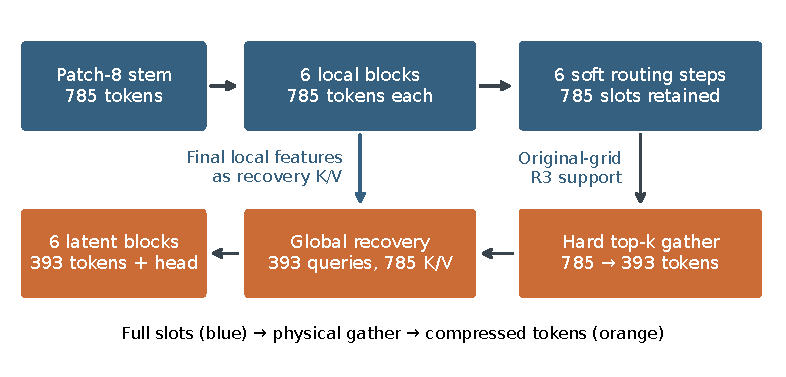
\includegraphics[width=\linewidth]{figures/architecture.pdf}
\caption{\mn{} at 224 pixels. Soft spatial transport keeps the full grid; the
exact-budget gather is the first physically shorter tensor. Recovery reads
the final full-grid local features, after which global reasoning uses 392
patch carriers. Counts exclude CLS.}
\label{fig:architecture}
\end{figure}

\subsection{Spatial mass routing}
Index patch $i$ by its original-grid coordinate $u_i$. At routing step
$\ell$, donor and receiver sets $A_\ell,B_\ell$ are disjoint, and donor $i$
may route only to
\begin{equation}
 \mathcal E_i^{(\ell)}(R)=\{j\in B_\ell:\|u_i-u_j\|_2\le R\}.
 \label{eq:support}
\end{equation}
The main model uses $R=3$. Coordinates stay tied to original slots throughout
routing. The global control removes this constraint; the flattened control
uses a width-8 window in row-major sequence order.

A learned $384\!\to\!64$ projection produces normalized metrics $z_i$. On
eligible edges,
\begin{equation}
 s_{ij}=\langle z_i,z_j\rangle/\tau,\quad
 q_{ij}=\frac{\exp s_{ij}}{\sum_{r\in\mathcal E_i}\exp s_{ir}},\quad
 a_{ij}=g_iq_{ij},
 \label{eq:routing}
\end{equation}
where $g_i$ is a soft donor decision. Following
\citet{sujianlin2024topk}, a monotone relaxation applies a data-dependent
threshold $\theta$ after sorting,
\begin{equation}
 g_i=F(\alpha\bar e_i-\theta),\qquad \sum_i g_i\approx k_\ell,
 \label{eq:softtopk}
\end{equation}
with row energy $e_i=\sum_j\exp s_{ij}$, $\alpha=30$, and the scheduled donor
budget $k_\ell$. This replaces serial top-$k$ decisions with a parallel soft
mask; it does not make the later gather indices differentiable.

Each slot carries mass $m_i$, initialized to one. A transport step preserves a
donor feature and transfers a fraction of its mass into receiver features:
\begin{align}
 m'_i&=m_i(1-\textstyle\sum_j a_{ij}), & X'_i&=X_i,\nonumber\\
 m'_j&=m_j+\textstyle\sum_i a_{ij}m_i, &
 X'_j&=\frac{m_jX_j+\sum_i a_{ij}m_iX_i}{m'_j}.
 \label{eq:transport}
\end{align}
The implementation clamps residual fractions and denominators. Sparse
neighbor lists restrict scored edges, but the released initialization still
constructs a dense adjacency buffer; our claim concerns learned routing
support, not linear memory for the whole implementation.

\subsection{Exact budget, recovery, and mass-aware attention}
For compression factor $\lambda$, the carrier count is
\begin{equation}
 K=N-\left\lfloor N(\lambda-1)/\lambda\right\rfloor.
 \label{eq:budget}
\end{equation}
The model hard-gathers the $K$ largest-mass patches. At $224^2$ and
$\lambda=2$, $N=784$ and $K=392$. A straight-through factor
$1+g-\operatorname{stopgrad}(g)$ on selected features sends gradients to the
continuous scores while hard indices execute the budget. Selected carriers
$Q$ then recover full-grid evidence through
\begin{equation}
 Y=Q+\operatorname{CrossAttn}(Q,H^{(6)},H^{(6)}),
 \label{eq:recovery}
\end{equation}
and six latent blocks process $K$ patches plus CLS.

Carrier mass enters latent attention as proportional attention:
\begin{equation}
 \operatorname{Attn}(Q,K,V;m)=
 \operatorname{softmax}\!\left(\frac{QK^\top}{\sqrt{d_h}}
 +\mathbf 1\log(m)^\top\right)V.
 \label{eq:mass-attn}
\end{equation}
The bias is rank one across queries. With
$\widehat Q=[Q,\sqrt{d_h}\mathbf1]$ and $\widehat K=[K,\log m]$, standard
scaled dot-product attention on $(\widehat Q,\widehat K,V)$ has exactly the
same logits. Padding the added head dimension to a multiple of eight lets the
released operator call unmodified FlashAttention. The reported ImageNet
checkpoints instead use PyTorch fused scaled-dot-product attention with an
additive mask; the FlashAttention path is validated separately by
forward/backward parity tests and is not credited with their runtime.
